
\chapter{Evaluation} 

\label{Chapter4}
In this chapter we elaborate the impact of the implemented changes on the performance.
Evaluating STM is worth a thesis itself. The biggest advantage of STM, the usability, is
its biggest disadvantage with regards to performance testing. STM is a universial tool. Most
synchronization problems can be solved with STM. This on the other hand means there
is no clear way to test STM, especially when measuring the performance. Thanks to
the moderate interface, testing the correct behaviour of STM is practicable. Testing 
is no guarantee that the implementation is correct in all regards, but it narrows the 
space for bugs. I wrote a number of small tests to test the implementations for specific bugs.
However, we will not investigate these correctness tests.


Unfortunately, testing the performance is extremely difficult. There are unlimited 
possibilities to use STM. Thus it is not possible to test the performance in general.
We can only test the performance for specific cases. This makes it hard to say which 
implementation has the best performance in general. To be able to classify the differnt 
tests and to compare the differnt test to each other, we use the following properties: 
\begin{itemize}
 \item costs of a transaction
 \item level of currency
\end{itemize}
The \keyword{costs} of a transaction denotes the time the transaction needs to execute when no 
other transaction is present.  
It is important to distinguish this from the time the transaction needs to execute. The
time heavily depends on other transactions. When a transaction is executed in a system
with many other transaction that work on the same TVars, the chance that it is rolled 
back is higher than if the transaction is the only transaction in the system. In our case 
we meassure the cost of a transaction by counting the \code{readTVar} and \code{writeTVar} 
operations. The costs of a transaction does not depend on the level of concurrency.

The \keyword{level of concurrency} denotes the density of the TVar usage. A high level of 
concurrency is givin if there are many transactions which are reading and writing the same
TVars. Read-only TVars are not considered, because reading them cannot result in a rollback.
Furthermore, if every transaction works on different TVars, there is no concurrency at all. If there 
is only one transaction, there is also no concurrency. Thus only if all three requirements are satisfied,
we speak of a high level of concurrency. This cannot be meassured in numbers, but we use this term
to compare different tests in a relative way.

These properties are not statically measurable in general because they often depend on the state of the TVars. 
The cost may vary depending on branches. The level of concurrency may also 
depend on branch conditions because it determines which TVars are accessed. Furthermore,
the scheduler does affect the level of concurrency. The GHC runtime system uses the \keyword{round robin}
scheduling scheme. If all transactions are sufficient cheap, they finish before their time expired.
This means irrespective of the number of threads, there is no concurrency at all (if a single OS thread
is used). To avoid these problems, the tests do not use branch contditions at all. Hence STMLA never rolls back.

\section{Test Setup}
Before we head over to the results, we will look upon the tests that are used to measure the performance.
I used basically two tests to compare the different implementations. The frist test is called \keyword{StmTest}.
It is used to test the performance and the correctness at the same time. StmTest has four parameters to control
the costs of a transaction and the level of concurrency:
\begin{itemize}
 \item \code{threads}
 \item \code{iterations}
 \item \code{tvars}
 \item \code{changes}
\end{itemize}
\code{threads} determines the number of threads that are working parallel. \code{iterations} is the number of transactions
each thread executes. \code{tvars} is the number of TVars that are created and used. \code{changes} is the number of write
operations per transaction. We use these parameters in the following as variables for integers.
StmTest starts by creating \code{tvars} TVars. Then \code{threads} threads are created. Each thread chooses \code{changes} TVars randomly from all 
created TVars (the same TVar may be chosen multiple times). Then the thread starts a transaction. In this transaction the thread reads each of chosen 
TVars, increments their value and writes the new value back to the TVar. This is repeated \code{iterations} times. When every forked thread has finished the
main thread reads all TVars an sums their values. If the STM system is correct, the sum is (\code{threads * iterations * changes}).

By altering the parameters the level of concurrency and the costs per transaction can be controlled. More \code{threads} and less 
\code{tvars} result in a higher level of concurrency. More \code{changes} mean not only higher costs of a transaction, but also
a higher level of concurrency. Unfortunately, in this test we are not able to increase the costs per transaction without increasing
the level of concurrency. The overall runtime of the test can be managed with \code{iterations}. It also helps to avoid that the thread
finishes before its round robin time expires. This test clarifies the previously mentioned problem of testing STM. These parameters can 
arbitrarily chosen and all of configurations are correct uses of STM. The number of combination on the other hand is nearly unlimited. Thus 
it is not possible to compare the implementations with all possible configurations. To determine which STM implementation is the best overall 
is anything but trivial.
Nevertheless, we use this test to compare the implementations on specific configurations to see their individuel strengths and weaknesses.
Note that the transactions in this test always write all the TVars they have read. This is not necessarily the case when STM is used in real programs. 
That is why, we use a second Test to meassure the performance.

\keyword{PerformanceTest} is a test to meassure the performance and not the correctness. In contrast to StmTest is has not four but
five parameters:
\begin{itemize}
 \item threads
 \item iterations
 \item tvars
 \item rWRatio
 \item writes
\end{itemize}
The first three parameters are the same as in StmTest. \code{rWRatio} determines the ratio between reads and writes. For example, if
the \code{rWRation} is \code{5}, the threads perform five reads for each write. \code{writes} on the other hands specifies
the number of writes that are executed in each transaction. This test allows us to increase the costs of the transactions by 
increasing the level of concurrency only slightly. If multiple transactions read the same TVar there is no conflict. If multiple
transaction on the other hand read and write the same TVar, there is a conflict. 

PerformanceTest ist similar to StmTest. It first creates \code{tvars} TVars. Then it forks \code{threads} threads. Each of these 
threads creates \code{writes} lists ramdomly with \code{rWRatio} TVars in each. For each inner list the transaction reads all TVars,
sums their values and writes them back to the first entry of that list. The list of lists is processed in a single transaction. 
This procedure is repeated \code{iterations} times. Since the TVars are choosen randomly, we cannot determine if the final state
of the TVars are correct after all threads are finished. Another difference between the two tests is that StmTest uses a list to 
store and lookup the TVars, while PerformanceTest uses an \code{IntMap}.

To meassure the execution time of the implementations the unix \code{time} command is used\footnote{\url{https://en.wikipedia.org/wiki/Time_(Unix)}}.
The test (either StmTest or PerformanceTest) are compiled with GHC 8.0.1\footnote{\url{https://www.haskell.org/ghc/download_ghc_8_0_1}} and the 
compiler flags \code{\-O2} for optimizations and \code{-threaded} to allow threaded runtime. The tests are exectued with the runtime option \code{-N} 
to allow multiple (in this case four) OS threads. The tests are executed on a system with an Intel(R) Core(TM) i7-6500U CPU @ 2.50GHz,
8GB @ 1600 Mhz DDR3 and a Fedora 25 OS. 


\section{Results}
Finally we inspect the results of the performance tests. I performed two series of tests to compare the different implementations.
In the first series the tests are configured by hand and the level of concurrency as well as the costs per transaction are modified.
The total workload was the same in all tests in this series. In the second test series the number of threads are increased in every
test. The workload per thread is unchanged and thus the total workload increases with the number of threads. 

\subsection{First Test Series}

\begin{figure}
\centering
 \begin{tabular}[center]{|c|c|c|c|c|}
  \hline
	                     & GHC    & Project & STMLA  & STMWSL \\ \hline
  StmTest(20,1000,200,050)   & 3.1780 &  3.5645 & 3.5340 & 3.6655 \\ \hline
  StmTest(20,2000,200,025)   & 3.3845 &  3.5700 & 3.6335 & 3.6665 \\ \hline
  StmTest(20,0500,200,100)   & 3.2978 &  3.8540 & 3.5905 & 3.7910 \\ \hline
  PerTest(20,500,200,10,10)  & 3.0420 &  3.2830 & 2.9225 & 3.4920 \\ \hline
  PerTest(20,500,200,20,05)  & 3.0670 &  3.3110 & 2.9425 & 3.4445 \\ \hline
  PerTest(20,500,200,05,20)  & 3.1520 &  3.4335 & 2.9455 & 3.3500 \\ \hline
 \end{tabular}
\caption[Runtime: Performance Tests]{Average runtime in seconds for tests with a total workload of 1.000.000 \code{readTVar} operations.}
\label{fig:results1}
\end{figure}

The results of the first test series are shown in Figure \ref{fig:results1}. 
The first column contains the test and its configuration.
StmTest(threads,iterations,tvars,changes) means the \code{StmTest} was applied with the previously explained configuration parameters.
PerTest(threads,iterations,tvars,rWRatio,writes) is the same for \code{PerformanceTest}. The first row introduces the different 
implementations. GHC is the current library in GHC 8. Project is the highlevel library that this thesis is based on.
STMLA and STMWSL are described in the previous chapter. For unknown reasons STMWSL performs poorly in this tests.\footnote{We 
analyze problems and potential performance issues of STMWSL in \ref{AppendixB}}

In the first three tests we examined how changes in the costs of a transaction effect the runtime of the four systems. 
The number of threads and TVars are fixed. By altering the \code{changes} parameter, we increase the workload per 
transaction. To preserve the total workload, we decrease the number of iterations each time we incease the number
of changes per transaction. In the first test we see that STMLA and the Project implementation perform equally good, while the GHC 
library performs slightly better and STMWSL slightly worse. In the second test the workload per transaction is halved compared to the
first test. The runtime of the GHC library and STMLA raises. Nevertheless, the GHC implementation is still the fastest. The increase 
in runtime can be explained with the fix overhead of each transaction. The second test executed twice as many transactions as
the first test, thus it needs to start and commit twice as many transactions.
The third test examines the other direction. The workload per transaction is doubled compared to the first test. 
This leads to an significant increase in runtime for the Project library and STMWSL. The GHC library becomes 
slightly slower with this configuration and STMLA remains on an equal level. This is the result we expected, since the rollback of 
a transaction is more expensive than in the first test. Fortunately, STMLA does not perform any rollback in this test. The Project
library on the otherhand performs rollbacks, which explains it increase in runtime. GHCs library also performs rollbacks
and thus its increase in runtime is only natural. We additionally increase the level of concurrency by increasing the 
TVars that each transaction accesses, which leads to more rollbacks in the GHC and Project libraries. This 

The last three tests use \code{PerformanceTest}. The number of reads per transaction are equal in all tests, but the 
\code{rWRatio} is different. The costs of a transaction are modified slightly, but the level of concurrency
is modified formidable. By increasing the number of writes (and preserving the total number of reads), we increase the costs of a transaction a little, but we 
increase the level of concurrency. The more TVars a transaction writes, the higher is the chance that another transaction is invalidated.
The first test executes ten writes
per transaction and ten reads for each write. The results are positive for STMLA since it is the fastest implementation.
STMWSL is the slowest implementation. The GHC implementation is slighty slower than STMLA but noticeable faster than the 
Project implementation. If we compare this to the second test, in which the number of reads remains the same, but the number of
writes is halved, no considerable changes are observable. All implementations remain on a similar level compared to the first
test. If we on the other hand increase the number of writes while retaining the number of reads as in the last test, the runtime of the
GHC and Project implementations are increasing. The runtime of STMLA remains similar to the two previous tests. 
Interesting is that0 the runtime of STMWSL is lower than before, but still not comparable to the runtime of STMLA.
This result is not surprising because the increase in concurrency does not effect STMLA. STMLA does not roll back at
all in this test and thus the configuration has no effect on the runtime. The GHC and Project implementation do
roll back. Hance a increase in runtime when increasing the level of concurrency is understandable.

While the results of the first three tests seem not very promising the alternative implementation, the results
of the last three tests reveal an application where STMLA outperforms even the GHC implementation. Even though the GHC implementation is 
an omptimized low level \code{C} implementation. 
More importantly, these tests met the expectations regarding the costs per transaction. First,
the performance does not decrease if we increase the costs per transaction. Since we do not execute any rollbacks in these 
tests, the costs per transaction do not matter for STMLA (and STMWSL). The GHC and Project library on the other hand 
lose performance in these cases. Second, the performance does not change if we increase the level of concurrency. By increasing
the level of concurrence the amount of rollbacks that are executed by the GHC and Project libraries increase. STMLA and STMWSL
on the other hand do not suffer from the increased level of concurrency. 
An explanation and a possible solution for the poor performance of STMWSL is givin in Chapter \ref{Chapter5}.


\subsection{Second Test Series}
We use the second test series to study the scalability of the implementations. We use \code{StmTest} as well as
\code{PerformanceTest} to compare the four implementations. Similar to the previous test series, the same test
is executed multiple times and the average execution time is meassured. The tests are randomized by the test themself 
and the scheduler. To get a representative result for the runtime, it is inevitable to execute the tests multiple 
times. To test the scalability we increased the number of threads over the course of the series. The other 
configuration parameters remained untouched in the whole test series. 
\begin{figure}
 \centering
 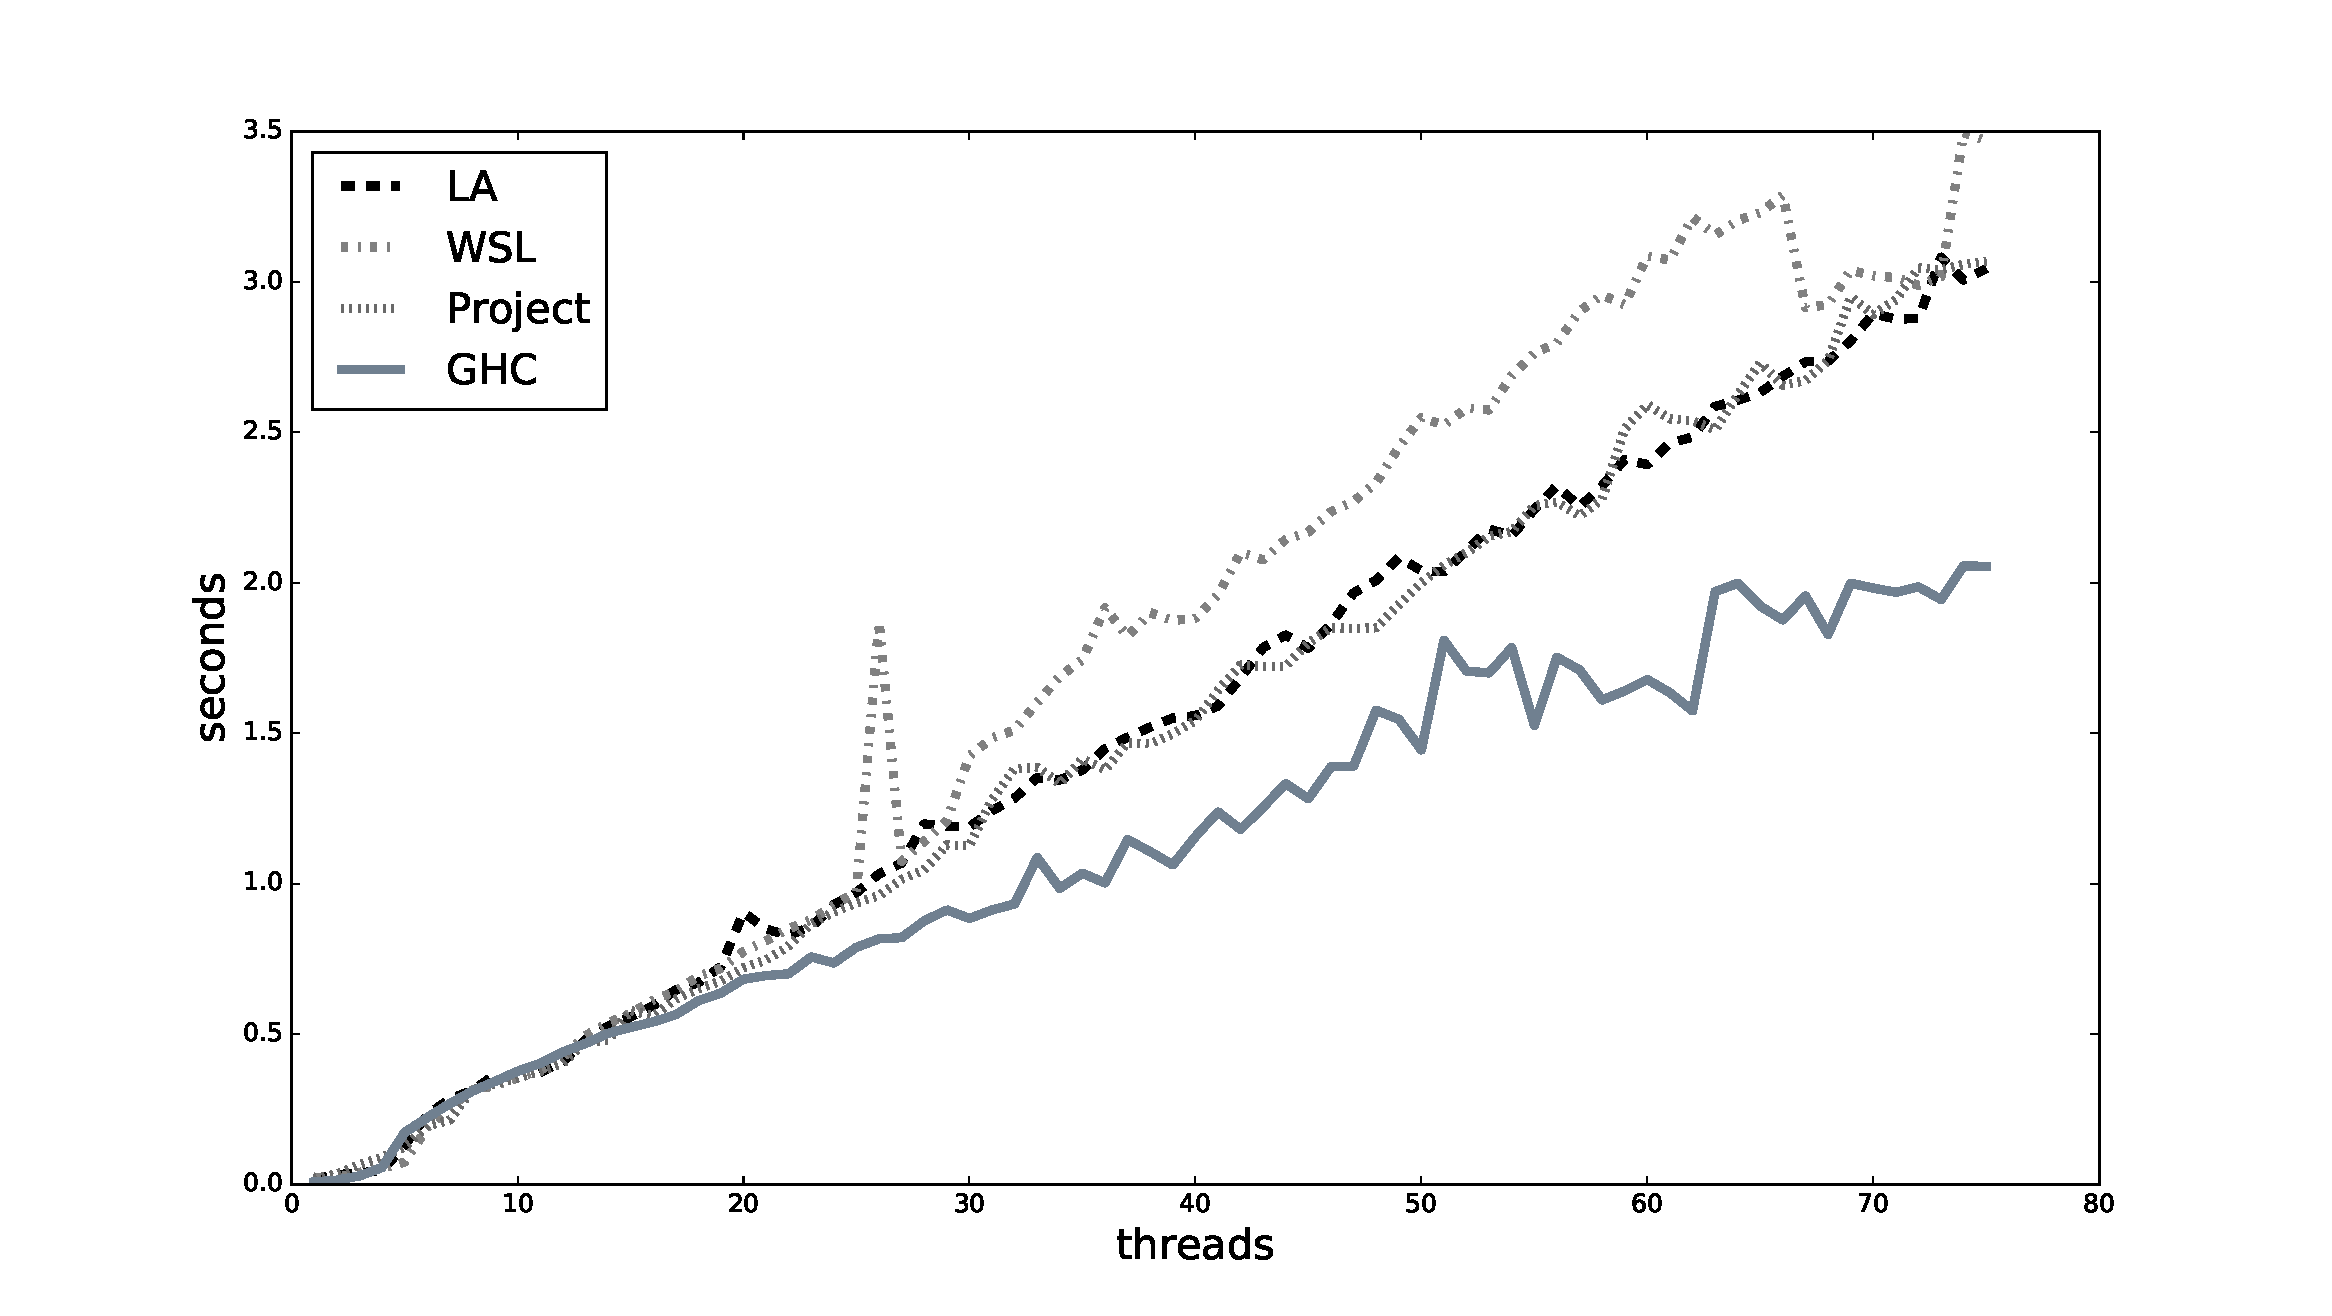
\includegraphics[scale=0.4]{Figures/Scaling1}
\caption[Runtime: Scaling Test I]{Results of the scaling tests with \code{StmTest}}
\label{fig:scaling1}
\end{figure}

Figure \ref{fig:scaling1} show the result of the scaling test performed with \code{StmTest}. We used the following 
configuration: 500 iterations per thread, 100 TVars stored in a list and 20 modifications per transactions with 
a varying number of threads. The x-axis describes the number of threads, while the y-axis contains the total runtime.
Note that an increase in threads results in an increased total work load. Thus the increase in runtime in all implementation
is mostly due to the increased total workload.
All implementations scale equally. The GHC implementation is slightly better and STMWSL is slightly worse than the other 
implementations. Overall, the runtime increases linear with number of threads. The GHC implementation stands out because of
its unstable execution time in this test series. Nevertheless, it still performs better than the other implementations.

\begin{figure}
 \centering
 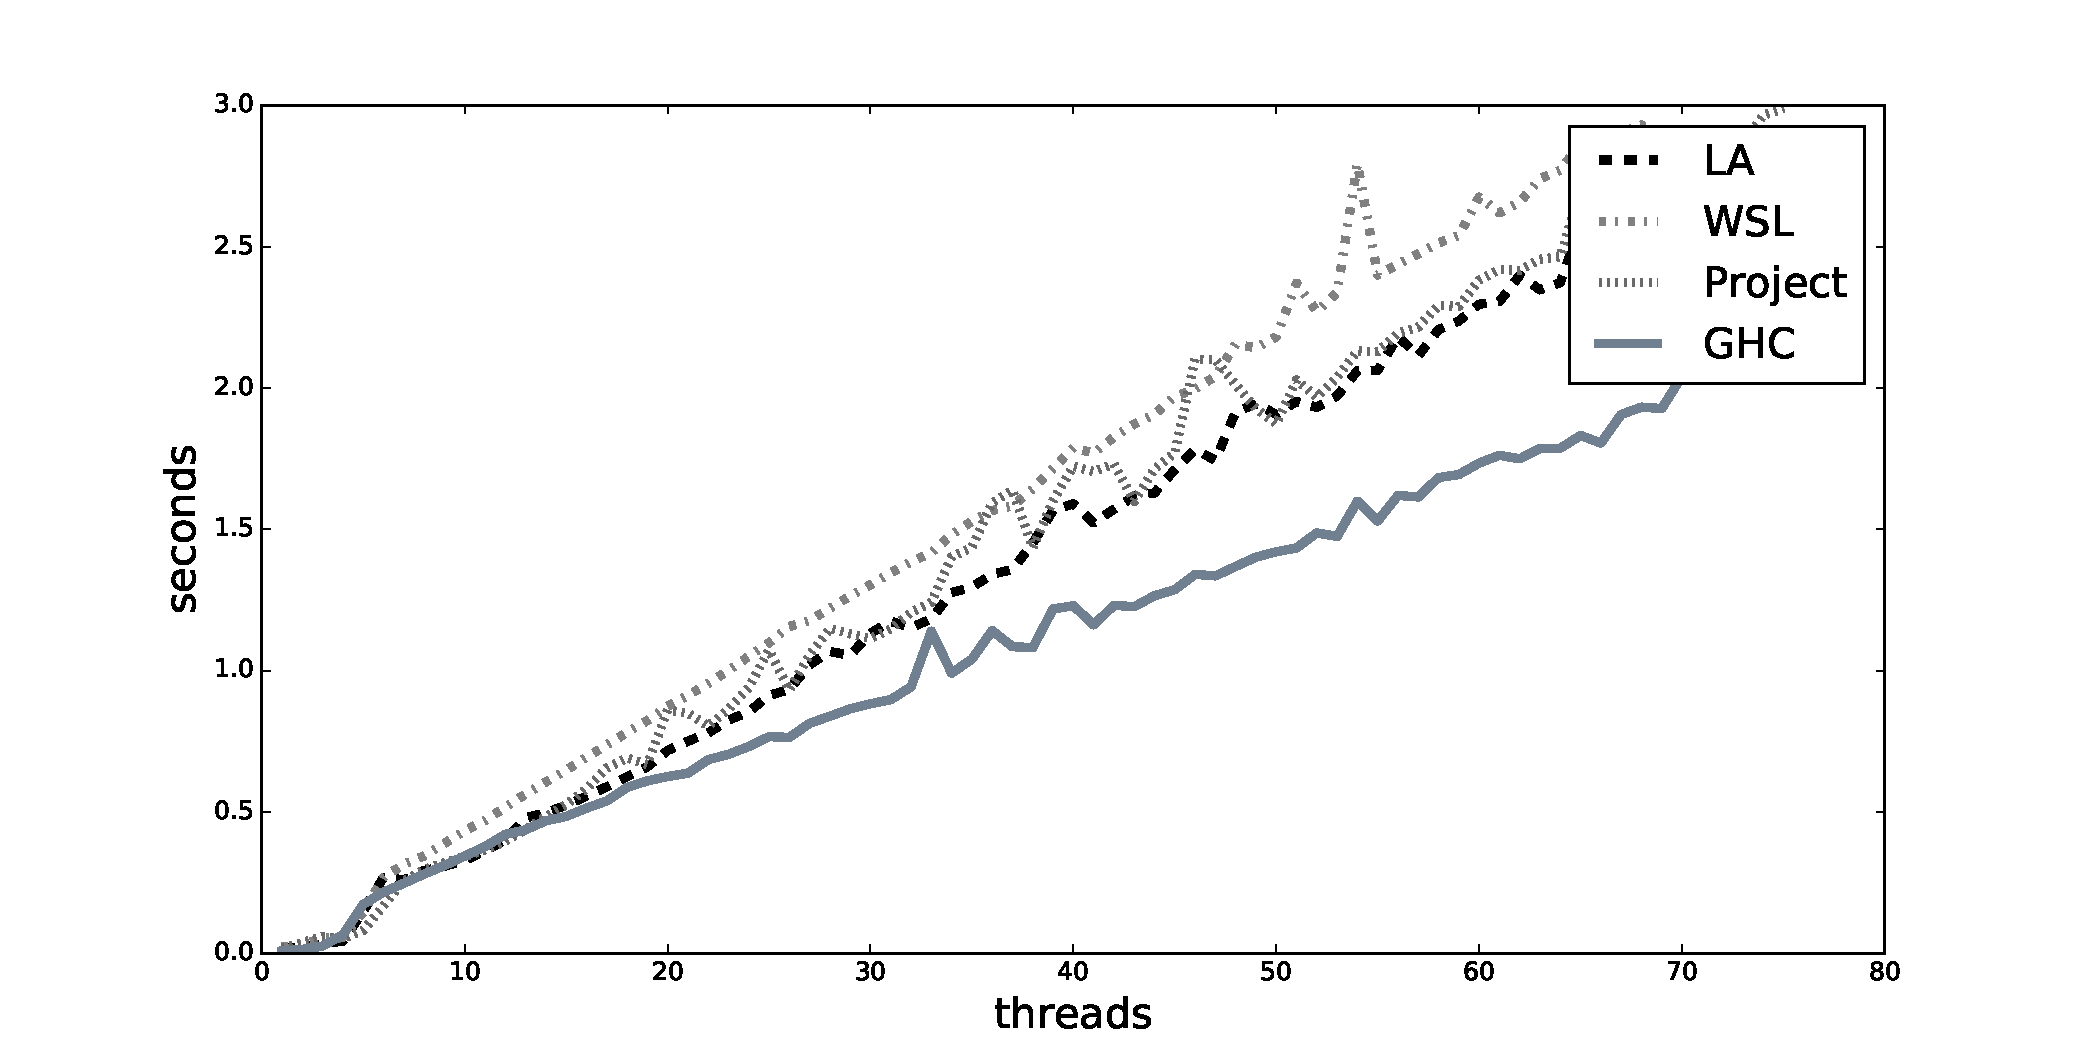
\includegraphics[scale=0.4]{Figures/Scaling2}
\caption[Runtime: Scaling Test II]{Results of the scaling tests with \code{PerformanceTest}}
\label{fig:scaling2}
\end{figure}

The results of the scaling tests performed with \code{PerformanceTest} are presented in Figure \ref{fig:scaling2}. The configuration 
is as follows: 500 transactions per thread, 200 TVar stored in an \code{IntMap}, five times more reads than write and
five writes per transaction (25 read operations per transaction). The results are similar to the previouse results. All implementation scale equally while
GHC is a slightly faster and STMWSL slightly slower. The jitter in the execution time of the GHC implementation are less noticable than 
in the first test. The execution time of the project implementation on the other hand varies much more in this test than
in the first test. Nonetheless, the general tendencies are not different. 

This test series show that all implementations are scalable. That GHC performs better than the highlevel implementations
is not surprising. In contrast to the tests presented in the previouse section, these test consist of small transactions.
The GHC implementation uses a very light weighted locking scheme. This makes the commit phase of the GHC implementation
significantly faster than the commit phase of the high level implementations. Thus the fixed (per transaction) overhead
of the highlevel implementations is higher than that of the GHC implementation. Since these tests use smaller transactions
than the first series, the results are reasonable.

\subsection{Observations}
While executing the tests, I noticed that the runtime option \code{N} that creates multiple OS threads slows down the 
computation as a whole. The runtime option \code{N} allows the user to specify the number of OS threads by adding a 
number. I performed some test with runtime options varying from \code{N1} to \code{N4} (since the processor contains four 
physical cores). The results are clear. The more OS thread the test uses the slower is the test. This is unpleasant 
because it means our efforts to utilize multi-core processors are futile. To avoid confusion, I am not saying that 
the computation is less efficient; it is slower. For example, one test takes 1.6 second when executed with \code{N1}
and the \textbf{same} test takes 2.3 seconds when executed with \code{N2} (2.6 with \code{N3} and 3.6 with \code{N4}).
The test consumed in the case of \code{N1} a singel core to its full extend (100\%). When the test runs with \code{N2},
it uses two cores, but not to their full extend (around 70\% per core). With \code{N3} it is about 50\% per core and 
with \code{N4} it is about 45\% per core. The system is not utilized by any other process (expect for the OS) while
testing. Even though the total amount of CPU consumption increases with the number of OS threads, the execution time 
as a whole slows down. I did not take any efforts to explore the reason for this. This is most likely a problem 
in the runtime systems and thus goes beyond the scope of this thesis. The fact remains that in this kind of
setup an increase in OS threads results in a decrease in performance. This \textit{kind of setup} is that most of 
the code is transactional code. Real worlds programs are usually not structured like these tests. The portion
of transactional code is far less. Hence this observation does not necessarily mean that STM is useless in 
practise. Nevertheless, all tests presented in this section are executed with \code{N4} to allow real parallelism. 

In addition to the performance test, I performed tests to check the implementations for memory leaks. The GHC implementation
as well as STMLA and STMWSL do not produce memory leaks as far as tested. The Project implementation on the other hand 
contains a memory leak. When ever a transaction reads a TVar, it enters its \code{retryMVar} to the queue of the TVar.
This allows other transactions to notify it in case they modify the TVar. If the TVar is never written, but continuously read, this queue grows
and is never emptied. The transactions themself do not remove the MVar from the queue when they rollback or commit.
This is for performance reasons because it requires the transaction to search for its own MVar in all TVar queues it 
has accessed. In STMWSL and STMLA the only time a transaction adds something to the queue is when it executes 
\code{retry}. Additionally, the transaction removes its MVar from the queue when it is no longer needed. In this 
case the performance is not as important as it is for the Project implementation. The \code{retry} either suspends 
the transaction and thus removing the MVars from the queues is a minor performance issue or it does not add the MVar to
the queue at all. The other entries of the TVar cannot produce any memory leaks because they only contain one entry
at a time. Since the log is discarded each time the transaction rolls back or successfully commits, no unused data is stored
within the log.